% ============================================================
%  THORN: Transport-Aligned Heterogeneous Observer-Routed
%         Neighborhood Attention
%
%  Research Paper — February 2026
% ============================================================
\documentclass[11pt,a4paper]{article}

% ---------- packages ----------
\usepackage[margin=1in]{geometry}
\usepackage{amsmath,amssymb,amsthm,mathtools}
\usepackage{algorithm}
\usepackage{algpseudocode}
\usepackage{booktabs}
\usepackage{graphicx}
\usepackage{xcolor}
\usepackage{hyperref}
\usepackage{cleveref}
\usepackage{enumitem}
\usepackage{multirow}
\usepackage{caption}
\usepackage{subcaption}
\usepackage{natbib}
\usepackage{tikz}
\usetikzlibrary{positioning, arrows.meta, fit, backgrounds, calc, decorations.pathreplacing}

\graphicspath{{../../artifacts/figures/}}

\hypersetup{
  colorlinks=true,
  linkcolor=blue!70!black,
  citecolor=green!50!black,
  urlcolor=blue!60!black,
}

% ---------- theorem environments ----------
\newtheorem{theorem}{Theorem}
\newtheorem{proposition}[theorem]{Proposition}
\newtheorem{corollary}[theorem]{Corollary}
\newtheorem{lemma}[theorem]{Lemma}
\newtheorem{remark}{Remark}
\newtheorem{definition}{Definition}

% ---------- macros ----------
\newcommand{\thorn}{\textsc{Thorn}}
\newcommand{\thornpp}{\textsc{Thorn++}}
\newcommand{\RR}{\mathbb{R}}
\newcommand{\EE}{\mathbb{E}}
\newcommand{\calM}{\mathcal{M}}
\newcommand{\calN}{\mathcal{N}}
\newcommand{\calL}{\mathcal{L}}
\newcommand{\bpi}{\boldsymbol{\pi}}
\newcommand{\boldA}{\mathbf{A}}
\DeclareMathOperator{\softmax}{softmax}
\DeclareMathOperator{\diag}{diag}

% ============================================================
\title{%
  \textsc{THORN}: Transport-Aligned Heterogeneous\\
  Observer-Routed Neighborhood Attention}

\author{%
  Richard Liu\\
  University of North Carolina at Charlotte\\
  \texttt{wliu23@charlotte.edu}
}

\date{February 2026}

% ============================================================
\begin{document}
\maketitle

% ============================================================
%  ABSTRACT
% ============================================================
\begin{abstract}
Graph attention networks route information using content-based
query-key similarity, ignoring the geometric structure of the graph
itself.
We propose \thorn{} (\textbf{T}ransport-aligned \textbf{H}eterogeneous
\textbf{O}bserver-\textbf{R}outed \textbf{N}eighborhood Attention),
which routes attention heads to competing graph views---feature-based,
temporal, and spectral---using geometric descriptors of local structure
(curvature, intrinsic dimension, density) rather than learned content
features.
A differentiable log-barrier mask continuously relaxes hard neighborhood
constraints, and a formal analysis reveals a previously uncharacterized
\emph{isolation-versus-interaction tradeoff}: mixing views before versus
after the attention softmax yields complementary strengths in different
data regimes.
On a controlled temporal-graph benchmark, post-softmax mixing achieves
0.984~PR-AUC / 0.992~ROC-AUC ($+6.5$ points over GAT) when one view
dominates, while pre-softmax mixing achieves 0.939~PR-AUC ($+2.0$
points over GAT) when views are complementary.
Ablation studies confirm that geometric observers---especially
curvature---carry routing signal that content features cannot replace:
removing curvature alone degrades performance by 7.5\%.
\thorn{} subsumes GAT, Graphormer, and MoE as special cases under
parameter-setting reductions.
\end{abstract}

% ============================================================
%  1. INTRODUCTION
% ============================================================
\section{Introduction}
\label{sec:intro}

Graph neural networks (GNNs) have become the dominant paradigm for
learning on relational data, with graph attention networks
\citep{velickovic2018graph, brody2022how} extending the transformer
attention mechanism \citep{vaswani2017attention} to irregular graph
topologies.
A key limitation of existing graph attention methods is their reliance on
\emph{content-based routing}: attention weights are computed solely from
learned query-key projections of node features, with graph structure
entering only as a binary mask that restricts the attention neighborhood.

This design has three fundamental shortcomings.
First, \textbf{hard neighborhood masks are non-differentiable} with
respect to topology, preventing end-to-end learning of which structural
connections should carry information.
Second, \textbf{content-only gating ignores geometric signals} such as
local intrinsic dimension, curvature, and density that carry direct
information about manifold structure and can serve as principled routing
priors.
Third, when multiple complementary graph views are available (e.g.,
feature-based $k$NN, temporal proximity, diffusion affinity),
\textbf{existing architectures lack a principled mechanism for
view-specific attention}, forcing a single set of query-key projections
to serve all structural perspectives simultaneously.

Graph transformers such as Graphormer \citep{ying2021transformers} and
GPS \citep{rampasek2022recipe} address part of this problem by
incorporating structural biases into attention, but they use fixed
encodings rather than learned, structure-aware routing.
Mixture-of-experts (MoE) architectures
\citep{shazeer2017outrageously, fedus2022switch} provide learned routing
but gate on content features alone, missing the geometric structure of
the graph.

We propose \thorn{}, which unifies these threads by introducing
\emph{observer-routed attention}: a mixture-of-experts router that gates
on geometric observer features---local intrinsic dimension (LID),
Ollivier--Ricci curvature, local outlier factor (LOF), and cross-view
consensus scores---to route each attention head to a specific graph view.
The selected views are combined via a log-barrier differentiable mask
that continuously relaxes hard neighborhood constraints while remaining
fully differentiable through the routing decisions.

\paragraph{Contributions.}
\begin{enumerate}[label=(\arabic*),nosep]
  \item \textbf{Geometric observer routing.}
    We introduce the first mechanism to route attention heads using
    manifold-geometric descriptors (curvature, intrinsic dimension,
    density) rather than content features.
    Ablation confirms these observers are non-redundant and that
    curvature alone accounts for a 7.5\% performance gap
    (\Cref{sec:routing,sec:observer_nonredundancy}).
  \item \textbf{Log-barrier differentiable masking.}
    We formalize a continuous relaxation of hard attention masks via a
    log-barrier with learned per-head temperature, enabling end-to-end
    gradient flow from task loss through routing to view selection
    (\Cref{prop:masking,sec:stability}).
  \item \textbf{Isolation-versus-interaction tradeoff.}
    We identify and formalize a fundamental tradeoff: mixing views
    before versus after the attention softmax yields complementary
    strengths.
    No single mode dominates; the optimal choice is predictable from
    the data's view correlation structure
    (\Cref{sec:pre_vs_post,sec:drift}).
  \item \textbf{Subsumption.}
    We show via function-class reductions that \thorn{} contains GAT,
    Graphormer, and MoE as special cases (\Cref{thm:subsumption}).
\end{enumerate}
We additionally explore extensions---view-specific projections and a
scalable alignment proxy---in \Cref{sec:view_projections,sec:online_proxy},
reporting both positive and negative results honestly.

% ============================================================
%  2. RELATED WORK
% ============================================================
\section{Related Work}
\label{sec:related}

\paragraph{Graph Neural Networks.}
Graph convolutional networks \citep{kipf2017semi} and graph isomorphism
networks \citep{xu2019powerful} aggregate neighbor features via fixed
or learnable weights but do not use attention.
GAT \citep{velickovic2018graph} introduced masked multi-head attention on
graphs, using a single-layer feedforward network to compute attention
coefficients.
GATv2 \citep{brody2022how} showed that the original GAT computes a
restricted form of \emph{static} attention and proposed a more expressive
dynamic formulation.
All of these methods use content-based scoring within a fixed neighborhood
defined by the input graph, with no mechanism for structure-aware
routing or multi-view integration.

\paragraph{Graph Transformers.}
Graphormer \citep{ying2021transformers} augments standard transformer
attention with structural encodings (shortest-path distances, degree
centrality) as additive biases, achieving strong results on molecular
property prediction.
GPS \citep{rampasek2022recipe} provides a general recipe combining local
message-passing with global attention and positional/structural
encodings.
These approaches use \emph{fixed} structural biases rather than
\emph{learned} structure-aware routing.

\paragraph{Mixture of Experts.}
The sparsely-gated MoE layer \citep{shazeer2017outrageously} and its
successor Switch Transformer \citep{fedus2022switch} route tokens to
expert subnetworks using content-based gating.
Load-balancing losses prevent expert collapse.
\thorn{} adapts the MoE paradigm to graph attention, replacing
content-based gating with geometric observer features and replacing
expert networks with graph views.

\paragraph{Optimal Transport on Graphs.}
Gromov--Wasserstein (GW) distance \citep{peyre2019computational}
provides a principled framework for comparing metric-measure spaces
without requiring shared feature spaces.
Fused GW (FGW) \citep{vayer2019optimal} jointly considers feature and
structural distances.
\thorn{} uses FGW to measure cross-view consistency and derive edge
consensus features for routing alignment.

\paragraph{Geometric Descriptors.}
Local intrinsic dimensionality \citep{levina2004maximum} estimates the
effective dimensionality of data near a point.
Ollivier--Ricci curvature \citep{ollivier2009ricci} measures the
convergence or divergence of geodesics and has been used for graph
rewiring and community detection;
Forman--Ricci curvature \citep{forman2003bochner} provides a scalable
combinatorial alternative.
\citet{topping2022understanding} connect curvature to over-squashing
in GNNs.
Local outlier factor \citep{breunig2000lof} quantifies the relative
density of a point's neighborhood.
Diffusion maps \citep{coifman2006diffusion} provide multi-scale
embeddings that capture the intrinsic geometry of data manifolds.
To our knowledge, \thorn{} is the first architecture to unify these
descriptors as observer features for dynamic attention routing.

\paragraph{Low-Rank Adaptation.}
LoRA \citep{hu2020lora} introduces low-rank additive adapters for
parameter-efficient fine-tuning of large models.
\thornpp{} adapts this idea to multi-view graph attention, using
per-view LoRA adapters on the shared $Q/K/V$ projections to enable
view-specific attention patterns with minimal parameter overhead.

% ============================================================
%  3. THORN ARCHITECTURE
% ============================================================
\section{\thorn{} Architecture}
\label{sec:arch}

\Cref{fig:architecture} provides a high-level overview of the \thorn{}
architecture, analogous to the Transformer diagram of
\citet{vaswani2017attention}.
The left column shows the full model pipeline from input node features
through $L$ stacked THORNBlocks to task prediction.
The right column expands the multi-view routed attention mechanism inside
each block, illustrating the two attention modes (pre-softmax and
post-softmax) and the flow of observer features through the MoE router.

\begin{figure}[t]
\centering
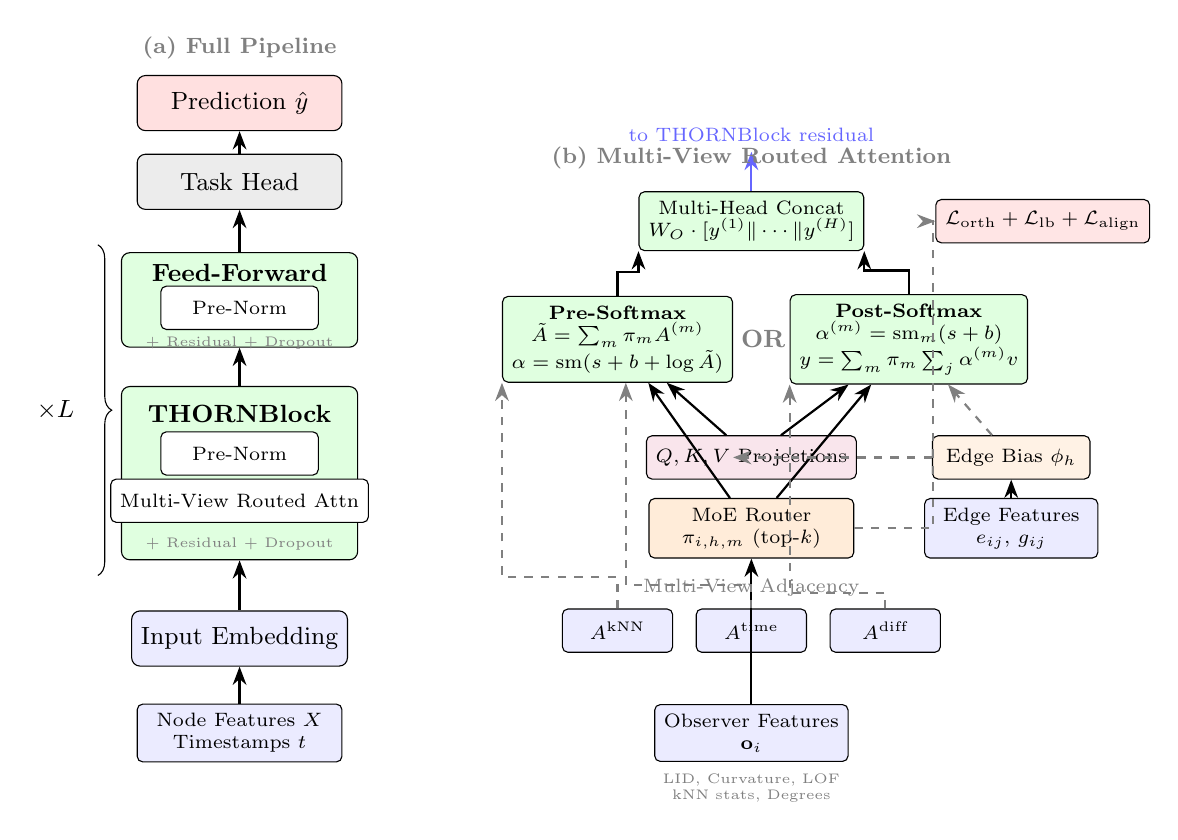
\begin{tikzpicture}[
  >=Stealth,
  block/.style={draw, rounded corners=3pt, minimum width=2.6cm,
    minimum height=0.7cm, align=center, font=\small},
  smallblock/.style={draw, rounded corners=2pt, minimum width=2.0cm,
    minimum height=0.55cm, align=center, font=\scriptsize},
  databox/.style={draw, rounded corners=2pt, fill=blue!8,
    minimum width=2.6cm, minimum height=0.55cm, align=center,
    font=\scriptsize},
  routerbox/.style={draw, rounded corners=2pt, fill=orange!15,
    minimum width=2.0cm, minimum height=0.55cm, align=center,
    font=\scriptsize},
  attnbox/.style={draw, rounded corners=2pt, fill=green!12,
    minimum width=2.0cm, minimum height=0.55cm, align=center,
    font=\scriptsize},
  lossbox/.style={draw, rounded corners=2pt, fill=red!10,
    minimum width=2.0cm, minimum height=0.55cm, align=center,
    font=\scriptsize},
  addnorm/.style={draw, circle, inner sep=1pt, font=\scriptsize,
    fill=yellow!20},
  arrow/.style={->, thick},
  darrow/.style={->, thick, dashed, gray},
  brace/.style={decorate, decoration={brace, amplitude=5pt, mirror}},
]

% ===== LEFT COLUMN: Full Pipeline =====
\node[databox] (input) at (0, 0) {Node Features $X$\\Timestamps $t$};
\node[block, fill=blue!8] (embed) at (0, 1.2) {Input Embedding};

% THORNBlock x L
\node[block, fill=green!12, minimum height=2.2cm, minimum width=3.0cm]
  (thornblock) at (0, 3.3) {};
\node[font=\small\bfseries] at (0, 4.05) {THORNBlock};
\node[smallblock, fill=white] (prenorm1) at (0, 3.55) {Pre-Norm};
\node[smallblock, fill=white] (mhra) at (0, 2.95) {Multi-View Routed Attn};
\node[font=\tiny, gray] at (0, 2.4) {+ Residual + Dropout};

\node[block, fill=green!12, minimum height=1.2cm, minimum width=3.0cm]
  (ffnblock) at (0, 5.5) {};
\node[font=\small\bfseries] at (0, 5.85) {Feed-Forward};
\node[smallblock, fill=white] (prenorm2) at (0, 5.4) {Pre-Norm};
\node[font=\tiny, gray] at (0, 4.95) {+ Residual + Dropout};

% Nx bracket
\draw[brace] (-1.8, 2.0) -- (-1.8, 6.2)
  node[midway, left=5pt, font=\small] {$\times L$};

\node[block, fill=gray!15] (taskhead) at (0, 7.0) {Task Head};
\node[block, fill=red!12] (output) at (0, 8.0) {Prediction $\hat{y}$};

% Arrows left column
\draw[arrow] (input) -- (embed);
\draw[arrow] (embed) -- (thornblock.south);
\draw[arrow] (thornblock.north) -- (ffnblock.south);
\draw[arrow] (ffnblock.north) -- (taskhead);
\draw[arrow] (taskhead) -- (output);

% ===== RIGHT COLUMN: Inside Routed Attention =====
\coordinate (rbase) at (6.5, -0.3);

% Observer features (offline)
\node[databox, minimum width=2.2cm] (obs) at (6.5, 0.0)
  {Observer Features\\$\mathbf{o}_i$};
\node[font=\tiny, gray, text width=2.5cm, align=center] at (6.5, -0.7)
  {LID, Curvature, LOF\\kNN stats, Degrees};

% Views
\node[databox, minimum width=1.4cm] (vknn) at (4.8, 1.3) {$A^{\text{kNN}}$};
\node[databox, minimum width=1.4cm] (vtime) at (6.5, 1.3) {$A^{\text{time}}$};
\node[databox, minimum width=1.4cm] (vdiff) at (8.2, 1.3) {$A^{\text{diff}}$};
\node[font=\scriptsize, gray] at (6.5, 1.85) {Multi-View Adjacency};

% Router
\node[routerbox, minimum width=2.6cm] (router) at (6.5, 2.6)
  {MoE Router\\$\pi_{i,h,m}$ (top-$k$)};
\draw[arrow] (obs) -- (router);

% Edge bias
\node[databox, minimum width=2.2cm] (edgefeat) at (9.8, 2.6)
  {Edge Features\\$e_{ij}$, $g_{ij}$};
\node[smallblock, fill=orange!10] (edgebias) at (9.8, 3.5)
  {Edge Bias $\phi_h$};
\draw[arrow] (edgefeat) -- (edgebias);

% Q, K, V
\node[smallblock, fill=purple!10, minimum width=2.6cm] (qkv) at (6.5, 3.5)
  {$Q, K, V$ Projections};

% Pre-softmax path
\node[attnbox, minimum width=2.6cm, minimum height=1.0cm] (presm)
  at (4.8, 5.0) {\textbf{Pre-Softmax}\\$\tilde{A} = \sum_m \pi_m A^{(m)}$\\
  $\alpha = \text{sm}(s + b + \log \tilde{A})$};

% Post-softmax path
\node[attnbox, minimum width=2.6cm, minimum height=1.0cm] (postsm)
  at (8.5, 5.0) {\textbf{Post-Softmax}\\$\alpha^{(m)} = \text{sm}_m(s + b)$\\
  $y = \sum_m \pi_m \sum_j \alpha^{(m)} v$};

% Routing arrows to attention modes
\draw[arrow] (router) -- (presm);
\draw[arrow] (router) -- (postsm);
\draw[arrow] (qkv) -- (presm);
\draw[arrow] (qkv) -- (postsm);
\draw[darrow] (edgebias) -- (presm.east |- edgebias);
\draw[darrow] (edgebias) -- (postsm);

% View arrows to attention
\draw[darrow] (vknn.north) -- ++(0, 0.4) -| (presm.south west);
\draw[darrow] (vtime.north) -- ++(0, 0.3) -| ([xshift=3pt]presm.south);
\draw[darrow] (vdiff.north) -- ++(0, 0.2) -| (postsm.south west);

% OR node
\node[font=\small\bfseries, gray] at (6.65, 5.0) {OR};

% Output aggregation
\node[attnbox, minimum width=2.6cm] (agg) at (6.5, 6.5)
  {Multi-Head Concat\\$W_O \cdot [y^{(1)} \| \cdots \| y^{(H)}]$};
\draw[arrow] (presm.north) -- ++(0, 0.3) -| (agg.south west);
\draw[arrow] (postsm.north) -- ++(0, 0.3) -| (agg.south east);

% Regularizers
\node[lossbox, minimum width=2.4cm] (regs) at (10.2, 6.5)
  {$\calL_{\text{orth}} + \calL_{\text{lb}} + \calL_{\text{align}}$};
\draw[darrow] (router.east) -- ++(1.0, 0) |- (regs);

% Connection arrow from right to left
\draw[arrow, blue!60, thick] (agg.north) -- ++(0, 0.5)
  node[above, font=\scriptsize, blue!60] {to THORNBlock residual};

% Title labels
\node[font=\footnotesize\bfseries, gray] at (0, 8.7) {(a) Full Pipeline};
\node[font=\footnotesize\bfseries, gray] at (6.5, 7.3)
  {(b) Multi-View Routed Attention};

\end{tikzpicture}
\caption{The \thorn{} architecture.
\textbf{(a)}~The full pipeline stacks $L$ THORNBlocks, each containing
multi-view routed attention followed by a feed-forward network, with
pre-norm residual connections throughout.
\textbf{(b)}~Inside routed attention: geometric observer features
$\mathbf{o}_i$ (LID, curvature, LOF, per-view degrees) feed an
MoE-style router that produces per-head routing probabilities
$\pi_{i,h,m}$ over $M$ graph views via top-$k$ gated softmax.
Two attention modes are available:
\emph{pre-softmax} (left) mixes view adjacencies before a single
softmax over the union neighborhood, enabling cross-view interaction;
\emph{post-softmax} (right) computes per-view attention independently
and combines outputs, preserving view isolation.
Edge observer features $e_{ij}$ (including FGW consensus $g_{ij}$)
provide per-head edge biases.
Auxiliary losses $\calL_{\mathrm{orth}}$, $\calL_{\mathrm{lb}}$, and
$\calL_{\mathrm{align}}$ regularize routing diversity, load balance,
and cross-view alignment respectively.
Compare with Figure~1 of \citet{vaswani2017attention}: \thorn{} replaces
single-graph self-attention with multi-view routed attention, and adds
the observer-driven routing pathway (orange) that has no analogue in
standard transformers.}
\label{fig:architecture}
\end{figure}

% ---- 3.1 Preliminaries ----
\subsection{Preliminaries and Notation}
\label{sec:prelim}

Let $G^{(m)} = (V, E^{(m)})$ denote the $m$-th neighborhood view over a
common node set $V$ with $|V| = N$, where
$m \in \calM = \{1, \ldots, M\}$ indexes views (e.g., $k$NN, temporal,
diffusion).
For each view, let $A^{(m)} \in \RR_{\ge 0}^{N \times N}$ be a weighted
adjacency matrix.
We write $i$ for the destination node and $j$ for a source neighbor;
attention weights satisfy
$\sum_{j \in \calN(i)} \alpha_{ij}^{(h)} = 1$
(the full attention formula is given in \Cref{eq:logbarrier}).
The union edge set is
$E_{\mathrm{union}} = \bigcup_{m \in \calM} E^{(m)}$.
Each node $i$ has feature vector $\mathbf{x}_i \in \RR^{d}$ and
optional timestamp $t_i \in \RR$.

% ---- 3.2 Observer Features ----
\subsection{Observer Features}
\label{sec:observers}

\thorn{} computes a set of \emph{observer features} $\mathbf{o}_i$ for
each node $i$ that characterize the local geometric and topological
structure.  These include:

\begin{itemize}[nosep]
  \item \textbf{Local intrinsic dimension (LID)}
    \citep{levina2004maximum}: estimated from $k$NN distances,
    characterizes the effective dimensionality near~$i$.
  \item \textbf{Ollivier--Ricci curvature} \citep{ollivier2009ricci}:
    measures convergence/divergence of random walks from neighboring
    nodes, indicating structural bottlenecks.
  \item \textbf{Local outlier factor (LOF)} \citep{breunig2000lof}:
    quantifies relative neighborhood density, identifying anomalous
    connectivity patterns.
  \item \textbf{$k$NN statistics}: mean and standard deviation of
    $k$-nearest-neighbor distances.
  \item \textbf{Temporal features}: normalized timestamp, temporal
    degree (number of temporal neighbors).
  \item \textbf{Per-view degree}: $\deg_i^{(m)}$ for each view $m$,
    providing a view-specific density signal.
\end{itemize}

For edges $(i, j)$, we additionally compute edge observer features
$e_{ij} = [d_{ij}^{\text{kNN}}, d_{ij}^{\text{time}},
d_{ij}^{\text{diff}}, \mathrm{LID}_i, \mathrm{LID}_j, g_{ij}]$,
where $g_{ij}$ is a cross-view consensus score derived from FGW
alignment (\Cref{sec:fgw}).

\paragraph{Scalable curvature via Forman--Ricci.}
Computing exact Ollivier--Ricci curvature requires solving a linear
program per edge, yielding $O(E \cdot N)$ complexity.
For scalability, we additionally provide Forman--Ricci curvature
\citep{forman2003bochner} as a drop-in alternative.
For an unweighted edge $(i, j)$:
\begin{equation}
  \label{eq:forman}
  F(i, j) = 4 - \deg(i) - \deg(j)
    + 3\,|\triangle_{ij}|,
\end{equation}
where $|\triangle_{ij}|$ is the number of triangles containing $(i, j)$.
Per-node curvature is the mean over incident edges.
Forman--Ricci captures over-squashing bottlenecks
\citep{topping2022understanding} with $O(E \cdot k_{\max})$ complexity,
where $k_{\max}$ is the maximum degree.

\subsubsection{Observer Non-Redundancy}
\label{sec:observer_nonredundancy}

A natural concern is whether the six observer feature families are
redundant---if LID, curvature, and LOF are highly correlated, the
router gains no additional signal from their combination.
We address this through three analyses (\Cref{tab:observer_analysis}):

\textbf{(i)~Correlation analysis.}
Pairwise Pearson and Spearman correlations across the standardized
observer feature vector show that only 2.8\% of feature pairs exceed
$|r| > 0.8$ (57 out of 2016 pairs).
The strongest correlations occur \emph{within} feature families
(specifically, multi-scale diffusion coordinates at different scales),
not \emph{across} them, confirming that each observer captures a
distinct geometric signal.

\textbf{(ii)~PCA effective rank.}
The Shannon entropy-based effective rank
$r_{\text{eff}} = \exp\!\big({-}\sum_k p_k \log p_k\big)$
(where $p_k = \lambda_k / \sum_j \lambda_j$ are the normalized PCA
eigenvalues) measures the effective dimensionality of the observer
feature space.
We observe $r_{\text{eff}} = 19.95$ out of 64 geometric observer
features (after standardization), with 22~PCs needed for 95\%
variance---indicating substantial independent variation across
observer families.

\textbf{(iii)~Observer ablation.}
The strongest validation comes from feature ablation
(\Cref{tab:observer_analysis}): zeroing each observer family and
measuring the PR-AUC degradation.
Curvature is the most critical individual observer ($-7.5\%$),
followed by view degrees ($-6.0\%$), LOF ($-1.4\%$), and LID
($-1.1\%$).
Removing all three geometric observers together (LID, curvature, LOF)
causes $-8.6\%$, confirming that these features collectively carry
the core routing signal.

% ---- 3.3 Multi-View Construction ----
\subsection{Multi-View Graph Construction}
\label{sec:views}

\thorn{} constructs $M = 3$ complementary graph views:

\paragraph{$k$NN view.}
Feature-space $k$-nearest neighbors with Gaussian kernel weights:
$A_{ij}^{\text{kNN}} = \exp(-\|x_i - x_j\|^2 / \sigma^2)$
for $j \in \text{kNN}(i)$.

\paragraph{Temporal view.}
Connects nodes within a time window with decay weights:
$A_{ij}^{\text{time}} = \exp(-|t_i - t_j| / \tau)$
for $|t_i - t_j| < \Delta t$.

\paragraph{Diffusion view.}
Multi-scale diffusion affinities derived from the graph Laplacian
eigenvectors \citep{coifman2006diffusion}:
$A_{ij}^{\text{diff}} = \sum_{k=1}^{K} \exp(-\lambda_k s)\,
\psi_k(i)\,\psi_k(j)$,
where $(\lambda_k, \psi_k)$ are eigenpairs of the normalized Laplacian
and $s$ is the diffusion timescale (not to be confused with node
timestamps $t_i$).

% ---- 3.4 MoE Routing ----
\subsection{MoE-Style Observer Routing}
\label{sec:routing}

The router produces per-node, per-head routing probabilities over views.
Unlike standard MoE which gates on content features, \thorn{} gates on
the observer feature vector $\mathbf{o}_i$:
\begin{equation}
  \label{eq:routing}
  \ell_{i,h,m} = W_h^{(3)} \cdot \mathrm{GELU}\!\big(
    W_h^{(2)} \cdot \mathrm{GELU}(
    W_h^{(1)} \cdot \mathrm{LN}(\mathbf{o}_i) + b_h^{(1)}
  ) + b_h^{(2)}\big) + b_h^{(3)} + \eta,
\end{equation}
where $\eta \sim \mathcal{N}(0, \sigma_{\text{noise}}^2)$ is Gaussian
exploration noise (training only) and $\mathrm{LN}$ is layer
normalization.
Routing probabilities are obtained via top-$k$ selection followed by
renormalized softmax:
\begin{equation}
  \label{eq:topk}
  \pi_{i,h,m} =
  \begin{cases}
    \frac{\exp(\ell_{i,h,m})}{\sum_{m' \in \text{top-}k}
      \exp(\ell_{i,h,m'})} & \text{if } m \in \text{top-}k(\ell_{i,h,\cdot}), \\
    0 & \text{otherwise}.
  \end{cases}
\end{equation}

The use of $k = 2$ (out of $M = 3$ views) allows each head to
specialize on a pair of views while maintaining sparse computation.

\subsubsection{View-Specific Projections (\thornpp{})}
\label{sec:view_projections}

A limitation of standard \thorn{} is that all views share the same
$Q$, $K$, $V$ projection matrices.
This creates a representational bottleneck: the shared projections must
simultaneously serve views with fundamentally different edge semantics
(feature similarity for $k$NN, temporal proximity for time, spectral
affinity for diffusion).

\thornpp{} addresses this via LoRA-style \citep{hu2020lora} low-rank
view-specific adapters.
For each view $m$, we define:
\begin{equation}
  \label{eq:lora_qkv}
  W_Q^{(m)} = W_Q + \Delta W_Q^{(m)}, \quad
  \Delta W_Q^{(m)} = B_Q^{(m)} A_Q^{(m)},
\end{equation}
where $A_Q^{(m)} \in \RR^{r \times d}$ (down-projection) and
$B_Q^{(m)} \in \RR^{d \times r}$ (up-projection), so
$\Delta W_Q^{(m)} \in \RR^{d \times d}$, with rank
$r = \lfloor d_h / 2 \rfloor$ (typically $r = 12$).
Analogous adapters are applied to $K$ and $V$.
The down-projections $A_Q^{(m)}$ use standard initialization while the
up-projections $B_Q^{(m)}$ are initialized to zero, ensuring that
$\Delta W_Q^{(m)} = 0$ at the start of training---the model begins
identical to shared-projection \thorn{} and gradually learns
view-specific deltas.

This adds $6Mrd$ parameters (3 for $Q/K/V$, each with a down- and
up-projection of size $r \times d$), a modest overhead ($< 5\%$)
relative to the shared projection parameters.
View-specific projections are used exclusively in post-softmax mode,
where each view's attention is computed independently and the projections
can specialize without interference.

% ---- 3.5 Log-Barrier Masking ----
\subsection{Log-Barrier Masking}
\label{sec:logbarrier}

\thorn{} combines the routing probabilities with view adjacency weights
to form a differentiable attention mask.
For each edge $(i, j) \in E_{\mathrm{union}}$, the routed edge weight
at destination $i$ from source $j$ is:
\begin{equation}
  \label{eq:routedA}
  \tilde{A}_{ij}^{(i,h)} = \sum_{m \in \calM}
    \pi_{i,h,m} \cdot A_{ij}^{(m)}.
\end{equation}

The attention logits incorporate this mask via a temperature-adaptive
log-barrier term:
\begin{equation}
  \label{eq:logbarrier}
  \alpha_{ij}^{(h)} = \softmax_{j}\!\Big(
    \underbrace{\frac{\langle q_i^{(h)}, k_j^{(h)} \rangle}{\sqrt{d}}}
      _{\text{content score } s_{ij}^{(h)}}
    + \underbrace{b_{ij}^{(h)}}_{\text{edge bias}}
    + \underbrace{\log\!\big(\tau_h \cdot \tilde{A}_{ij}^{(i,h)}
      + \epsilon\big)}_{\text{adaptive log-barrier mask}}
  \Big),
\end{equation}
where $b_{ij}^{(h)} = \phi_h(e_{ij})$ is a per-head edge bias computed
by a small MLP from edge observer features, $\epsilon > 0$ is a
numerical stabilizer, and $\tau_h = \mathrm{softplus}(s_h)$ is a
\emph{learned per-head temperature} with $s_h$ initialized to
$\mathrm{softplus}^{-1}(1) \approx 0.5413$ so that $\tau_h = 1$
at initialization.

\paragraph{Adaptive temperature motivation.}
The original log-barrier $\log(\tilde{A}_{ij} + \epsilon)$ is
numerically fragile when edge weights are compressed by graph
normalization (e.g., symmetric normalization maps soft Gaussian weights
from $[0, 1]$ to $[0.01, 0.3]$, causing
$\log(0.01) \approx -4.6$ to dominate content scores).
The learned temperature $\tau_h$ insulates the barrier from
normalization-induced compression: after a few gradient steps, each head
learns a $\tau_h$ that rescales its barrier contribution to the
appropriate dynamic range.
This eliminates the need to avoid normalization entirely---$\tau_h$ acts
as an automatic calibration mechanism
(\Cref{tab:stability}).

\begin{proposition}[Continuous relaxation of sparse masking]
  \label{prop:masking}
  Assume $\tilde{A}_{ij}^{(i,h)} \in [0, 1]$ and $\epsilon \downarrow 0$.
  Then \eqref{eq:logbarrier} is a continuous relaxation of discrete
  sparse attention: if $\tilde{A}_{ij}^{(i,h)} = 0$ then
  $\alpha_{ij}^{(h)} \to 0$, while if $\tilde{A}_{ij}^{(i,h)} > 0$ then
  $\alpha_{ij}^{(h)}$ is well-defined and differentiable with respect to
  $\tilde{A}_{ij}^{(i,h)}$.
\end{proposition}

\begin{proof}
  If $\tilde{A}_{ij}^{(i,h)} \to 0$, then
  $\log(\tilde{A}_{ij}^{(i,h)} + \epsilon) \to -\infty$, so
  $\exp(s_{ij}^{(h)} + b_{ij}^{(h)} +
  \log(\tilde{A}_{ij}^{(i,h)} + \epsilon)) \to 0$
  and the softmax assigns vanishing mass to edge $(i, j)$.
  If $\tilde{A}_{ij}^{(i,h)} > 0$, then the log term is finite and
  smooth; since softmax is smooth, $\alpha_{ij}^{(h)}$ is differentiable
  in $\tilde{A}_{ij}^{(i,h)}$ and therefore in routing logits
  $\ell_{i,h,m}$ through \eqref{eq:routedA}.
\end{proof}

\paragraph{Relation to prior work.}
GAT \citep{velickovic2018graph} enforces sparsity by restricting
$j \in \calN(i)$ via hard indexing.
Transformers commonly mask by adding $-\infty$ to disallowed logits.
The log-barrier formulation retains the semantics of hard masking while
remaining fully differentiable with respect to routing and view mixing,
enabling end-to-end gradient flow from the task loss through the router
to the view selection.

% ---- 3.6 Pre- vs Post-Softmax ----
\subsection{Pre-Softmax vs.\ Post-Softmax View Mixing}
\label{sec:pre_vs_post}

A key architectural choice in multi-view attention is \emph{where} the
routing-weighted combination of views occurs relative to the attention
softmax.
We formalize two modes and show they capture fundamentally different
inductive biases.

\paragraph{Pre-softmax mixing (``bias'' mode).}
Views are combined \emph{before} the attention softmax, allowing
cross-view interaction in the attention distribution:
\begin{align}
  \tilde{A}_{ij}^{(i,h)} &= \sum_{m} \pi_{i,h,m} \cdot A_{ij}^{(m)},
  \label{eq:presoftmax_A} \\
  \alpha_{ij}^{(h)} &= \softmax_{j \in \calN_{\mathrm{union}}(i)}\!\Big(
    s_{ij}^{(h)} + b_{ij}^{(h)} +
    \log\big(\tau_h \cdot \tilde{A}_{ij}^{(i,h)} + \epsilon\big)\Big),
  \label{eq:presoftmax_attn} \\
  y_i^{(h)} &= \sum_{j \in \calN_{\mathrm{union}}(i)}
    \alpha_{ij}^{(h)} \cdot v_j^{(h)}.
  \label{eq:presoftmax_agg}
\end{align}
Here, the softmax normalizes over the \emph{entire} union neighborhood.
An edge appearing in multiple views with high routing weight accumulates
mass, enabling cross-view synergy.
However, views with more edges can dilute the attention of sparser views,
and the shared $Q/K/V$ projections must serve all views simultaneously.

\paragraph{Post-softmax mixing (``post\_softmax'' mode).}
Each view computes its own attention distribution independently, and
routing combines the \emph{outputs}:
\begin{align}
  \alpha_{ij}^{(h,m)} &= \softmax_{j \in \calN^{(m)}(i)}\!\Big(
    s_{ij}^{(h)} + b_{ij}^{(h,m)}\Big),
  \label{eq:postsoftmax_attn} \\
  y_i^{(h)} &= \sum_{m} \pi_{i,h,m} \sum_{j \in \calN^{(m)}(i)}
    \alpha_{ij}^{(h,m)} \cdot v_j^{(h)}.
  \label{eq:postsoftmax_agg}
\end{align}
Each view's softmax normalizes only over its own neighborhood, preventing
cross-view dilution.
The dominant view's signal is preserved at full strength.
However, cross-view interaction is lost: the model cannot discover that
an edge present in multiple views is more trustworthy.

\paragraph{The isolation-versus-interaction tradeoff.}
These two modes represent endpoints of a fundamental tradeoff:
\begin{itemize}[nosep]
  \item \textbf{Isolation} (post-softmax): prevents interference,
    preserves pure signals, optimal when one view dominates.
  \item \textbf{Interaction} (pre-softmax): enables synergy, discovers
    cross-source patterns, optimal when views are complementary.
\end{itemize}
The optimal choice depends on the data's \emph{view correlation
structure}: high cross-view redundancy favors post-softmax (avoids
dilution), while high cross-view complementarity favors pre-softmax
(exploits synergy).
Our experiments (\Cref{sec:drift}) provide the first systematic
empirical demonstration of this tradeoff.

\paragraph{Why post-softmax achieves 0.984 PR-AUC.}
To understand why post-softmax mixing can dramatically outperform
pre-softmax in certain regimes, consider the information-theoretic
dynamics of each mode.
At drift${} = 0.50$, the temporal view provides a near-perfect
classification signal: nodes close in time share labels with high
probability, and the moderate drift means temporal features encode class
boundaries cleanly.
The $k$NN and diffusion views, constructed from the full 16-dimensional
feature space (13 noise dimensions, 3 signal dimensions), carry
substantially more noise than signal at this drift level.

In \textbf{pre-softmax} mixing, the attention softmax normalizes over
the \emph{entire union neighborhood} $\calN_{\mathrm{union}}(i)$.
Every edge from every view competes for the same probability mass.
Even when the router assigns high weight to the temporal view
($\pi_{\text{time}} \approx 0.87$), the $k$NN edges are not fully
suppressed---they retain residual weight through the log-barrier term
$\log(\tilde{A}_{ij} + \epsilon)$ and still consume attention mass.
With 13 noise dimensions driving $k$NN edge construction, these
residual edges inject noise into the attention distribution.
The shared $Q/K/V$ projections compound this problem: they must
simultaneously serve temporal edges (where proximity in time matters)
and $k$NN edges (where feature similarity matters), creating a
representation conflict.
The net effect is a ceiling of 0.920~PR-AUC---the architecture cannot
fully exploit the clean temporal signal because noisy cross-view edges
dilute it.

In \textbf{post-softmax} mixing, each view computes its own attention
distribution with a \emph{view-local} softmax:
$\alpha_{ij}^{(h,m)} = \softmax_{j \in \calN^{(m)}(i)}(s_{ij}^{(h)} +
b_{ij}^{(h,m)})$.
The temporal view's softmax normalizes only over temporal neighbors,
producing a clean, noise-free attention distribution.
The $k$NN view's noisy attention is computed separately and receives
low routing weight ($\pi_{\text{kNN}} \approx 0.13$), so its noise
contribution to the final output
$y_i^{(h)} = \sum_m \pi_{i,h,m} \sum_j \alpha_{ij}^{(h,m)} v_j^{(h)}$
is multiplicatively suppressed.
This isolation allows the temporal signal to flow at full fidelity,
yielding 0.984~PR-AUC and 0.992~ROC-AUC.

\paragraph{Why pre-softmax achieves 0.939 PR-AUC when views are
complementary.}
At drift${} = 0.75$, the data undergoes a \emph{regime shift} at
normalized time $t_n = 0.75$: labels receive a $+1.125$ logit boost
for late-arriving nodes, and cluster centers have drifted significantly.
This creates a scenario where no single view is sufficient.
Temporal edges connect nodes within the same time window, but the regime
shift means that early and late nodes have fundamentally different
class distributions---temporal proximity alone cannot resolve the
boundary.
Meanwhile, $k$NN edges group nodes by feature similarity \emph{across}
time, connecting early and late nodes that share similar features but
different labels.
This cross-temporal grouping provides information that temporal edges
cannot: it reveals which feature patterns persist versus which are
regime-dependent.

Pre-softmax mixing captures this complementarity because the union
softmax allows $k$NN edges and temporal edges to jointly shape the
attention distribution.
An edge $(i, j)$ that appears in \emph{both} the $k$NN and temporal
views accumulates routing weight from both
($\tilde{A}_{ij} = \pi_{\text{kNN}} \cdot A_{ij}^{\text{kNN}} +
\pi_{\text{time}} \cdot A_{ij}^{\text{time}}$), creating a natural
\emph{cross-view reinforcement} signal.
Edges supported by multiple views are more likely to connect
same-class nodes, and pre-softmax mixing exploits this by assigning
them higher attention weight after the log-barrier transformation.
Post-softmax mixing, by contrast, computes separate attention
distributions per view and cannot discover that cross-view edge
agreement is informative---it treats each view as an independent
information source, missing the synergy.

\paragraph{Formal characterization.}
Let $\calN^{(m)}(i)$ denote view $m$'s neighborhood of node $i$ and
$\calN_\cup(i) = \bigcup_m \calN^{(m)}(i)$ the union.
Define the \emph{view overlap ratio}
$\rho_i = |\bigcap_m \calN^{(m)}(i)| / |\calN_\cup(i)|$
and the \emph{signal-to-noise ratio} of view $m$ as
$\mathrm{SNR}_m = \mathrm{Var}[\text{signal features}] /
\mathrm{Var}[\text{noise features}]$ within $\calN^{(m)}(i)$.
Then:
\begin{itemize}[nosep]
  \item When $\max_m \mathrm{SNR}_m \gg \mathrm{SNR}_{m'}$ for
    $m' \neq m$ (one view dominates), post-softmax preserves the
    dominant view's clean attention while multiplicatively suppressing
    noisy views via $\pi_{i,h,m'} \approx 0$.
  \item When $\rho_i$ is high and $\mathrm{SNR}_m$ values are
    comparable (views are complementary), pre-softmax enables
    cross-view reinforcement through the additive log-barrier:
    $\log(\sum_m \pi_m A^{(m)}_{ij} + \epsilon) >
    \max_m \log(\pi_m A^{(m)}_{ij} + \epsilon)$ for shared edges.
\end{itemize}
This characterization predicts the empirical results in
\Cref{tab:drift}: at drift${} = 0.50$, the temporal view has
$\mathrm{SNR}_{\text{time}} \gg \mathrm{SNR}_{\text{kNN}}$, favoring
post-softmax isolation; at drift${} = 0.75$, the regime shift
equalizes view informativeness and increases $\rho_i$, favoring
pre-softmax interaction.

% ---- 3.7 FGW Alignment ----
\subsection{Fused Gromov--Wasserstein Cross-View Alignment}
\label{sec:fgw}

To encourage routing consistency across views, \thorn{} computes
Fused Gromov--Wasserstein (FGW) \citep{vayer2019optimal} alignment
between ego-neighborhoods in different views.
FGW jointly considers feature distances
$\|x_i - x_j\|$ and structural distances (shortest-path or diffusion
distance) to produce a transport plan $T^{(m, m')}$ between views
$m$ and $m'$ at each node.

The resulting transport plans are cached as edge consensus features:
\begin{equation}
  g_{ij} = \frac{1}{\binom{M}{2}} \sum_{m < m'} T_{ij}^{(m,m')},
\end{equation}
which are included in the edge observer features $e_{ij}$ and used
in the per-head edge bias $b_{ij}^{(h)} = \phi_h(e_{ij})$.
Additionally, per-node discordance scores
$D_{i,m} = 1 - \text{confidence}_{i,m}$ are used in the alignment
regularizer (\Cref{sec:regularizers}).

The FGW computation uses the Sinkhorn algorithm for entropic
regularization combined with Frank--Wolfe optimization for the
structural component \citep{peyre2019computational}.
Transport is computed \emph{offline} on ego-neighborhoods
and cached, avoiding $O(N^3)$ runtime during training.

\subsubsection{Online Alignment Proxy (\thornpp{})}
\label{sec:online_proxy}

Full FGW alignment is $O(N^3)$ per view pair, limiting its
applicability to inductive and streaming settings where the graph
evolves.
\thornpp{} introduces an online alignment proxy with $O(E)$ complexity
\citep{scetbon2022linear} that combines two complementary signals:

\textbf{(1)~Neighborhood Jaccard overlap.}
For each node $i$, the structural agreement between views $a$ and $b$
is measured by the Jaccard index of their neighborhoods:
\begin{equation}
  \label{eq:jaccard}
  J_i = \frac{|\calN^{(a)}(i) \cap \calN^{(b)}(i)|}
    {|\calN^{(a)}(i) \cup \calN^{(b)}(i)|}.
\end{equation}
This captures whether the two views agree on local connectivity---a
purely structural signal computed in $O(\deg_a(i) + \deg_b(i))$ per node.

\textbf{(2)~Neighbor feature distribution similarity.}
We compare the mean neighbor feature vectors across views via cosine
similarity:
\begin{equation}
  \label{eq:feat_sim}
  S_i^{\text{feat}} = \frac{1}{2}\left(
    1 + \cos\!\Big(\bar{x}_i^{(a)},\; \bar{x}_i^{(b)}\Big)
  \right),
  \qquad
  \bar{x}_i^{(m)} = \frac{1}{\deg_m(i)}
    \sum_{j \in \calN^{(m)}(i)} x_j.
\end{equation}
This captures feature-distributional agreement: views whose neighborhoods
contain similar features are more likely to be structurally consistent.

The combined overlap score is $O_i = 0.6\, J_i + 0.4\, S_i^{\text{feat}}$,
weighting structural agreement more heavily.
This proxy is fully differentiable (through the feature term),
recomputable on-the-fly for evolving graphs, and serves the same role
as FGW consensus in the edge observer features.

% ---- 3.8 THORNBlock ----
\subsection{THORNBlock Architecture}
\label{sec:thornblock}

\thorn{} stacks $L$ identical blocks (default $L = 3$), each following
the pre-norm transformer convention:
\begin{align}
  \hat{\mathbf{h}}_i^{(\ell)} &= \mathbf{h}_i^{(\ell-1)} +
    \mathrm{Dropout}\!\Big(
      W_O \cdot \mathrm{Concat}_{h=1}^{H}\, y_i^{(\ell, h)}
    \Big),
  \label{eq:block_attn} \\
  \mathbf{h}_i^{(\ell)} &= \hat{\mathbf{h}}_i^{(\ell)} +
    \mathrm{Dropout}\!\Big(
      \mathrm{FFN}\!\big(\mathrm{LN}(\hat{\mathbf{h}}_i^{(\ell)})\big)
    \Big),
  \label{eq:block_ffn}
\end{align}
where $y_i^{(\ell, h)}$ is the attention output from \Cref{sec:logbarrier}
or \Cref{sec:pre_vs_post}, queries/keys/values are projected from
$\mathrm{LN}(\mathbf{h}_i^{(\ell-1)})$, and $\mathrm{FFN}$ is a
two-layer network with GELU activation and expansion ratio~4.

The pre-norm residual connections serve a dual purpose: stabilizing deep
training and providing implicit self-information preservation, which
renders explicit self-loops in the graph unnecessary (see
\Cref{sec:theory_vs_practice}).

% ---- 3.9 Regularizers ----
\subsection{Regularizers}
\label{sec:regularizers}

\thorn{} employs three auxiliary losses to prevent routing collapse and
encourage structural alignment:

\paragraph{Head-view orthogonality ($\calL_{\mathrm{orth}}$).}
Let $P_i \in \RR^{H \times M}$ be the routing matrix at node $i$ with
entries $\pi_{i,h,m}$.
To prevent all heads from selecting the same view:
\begin{equation}
  \label{eq:lorth}
  \calL_{\mathrm{orth}} = \lambda_{\mathrm{orth}}
    \sum_{i=1}^{N} \left\lVert
      \frac{P_i P_i^\top}{\|P_i\|_F^2}
      - \frac{I_H}{H}
    \right\rVert_F^2.
\end{equation}
This pushes the normalized Gram matrix of routing vectors toward a
scaled identity, encouraging orthogonal head specialization.
Empirically, $\lambda_{\mathrm{orth}} = 5 \times 10^{-3}$ is optimal
(\Cref{sec:theory_vs_practice}).

\paragraph{Load balancing ($\calL_{\mathrm{lb}}$).}
Following the Switch Transformer \citep{fedus2022switch}, we penalize
uneven global view usage:
\begin{equation}
  \label{eq:llb}
  \calL_{\mathrm{lb}} = \lambda_{\mathrm{lb}}
    \sum_{m=1}^{M} \left( u_m - \frac{1}{M} \right)^2,
  \qquad
  u_m = \frac{1}{NH} \sum_{i,h} \pi_{i,h,m}.
\end{equation}

\paragraph{Alignment regularization ($\calL_{\mathrm{align}}$).}
Using the FGW-derived discordance scores $D_{i,m}$:
\begin{equation}
  \label{eq:lalign}
  \calL_{\mathrm{align}} = \lambda_{\mathrm{align}}
    \sum_{i,h,m} \pi_{i,h,m}\, D_{i,m}.
\end{equation}
This penalizes routing probability mass on views with high discordance,
pushing the router toward structurally consistent views.

\paragraph{Total loss.}
\begin{equation}
  \label{eq:totalloss}
  \calL = \calL_{\mathrm{task}} + \calL_{\mathrm{orth}}
    + \calL_{\mathrm{lb}} + \calL_{\mathrm{align}}.
\end{equation}

% ---- 3.10 Algorithm ----
\subsection{Algorithm}
\label{sec:algorithm}

\Cref{alg:thorn} provides the complete \thorn{} forward pass.

\begin{algorithm}[t]
\caption{\thorn{}: Forward Pass}
\label{alg:thorn}
\begin{algorithmic}[1]
\Require Node features $X \in \RR^{N \times d_0}$, timestamps
  $t \in \RR^{N}$, views $\calM = \{\text{kNN}, \text{time},
  \text{diff}\}$, depth $L$, heads $H$
\Statex
\State \textbf{Offline:} Build $A^{(m)}$, compute observer features
  $\mathbf{o}_i$, edge features $e_{ij}$, FGW consensus $g_{ij}$,
  discordance $D_{i,m}$
\State Form $E_{\mathrm{union}} = \bigcup_m E^{(m)}$
\Statex
\State $\mathbf{H}^{(0)} \gets \mathrm{Embed}(X)$
  \Comment{$N \times d$}
\For{$\ell = 1$ to $L$}
  \State $Q, K, V \gets$ projections from
    $\mathrm{LN}(\mathbf{H}^{(\ell-1)})$
    \Comment{$N \times H \times d_h$}
  \State $\pi_{i,h,m} \gets \text{top-}k\text{-softmax}\big(
    f_{\text{route}}(\mathbf{o}_i)\big)$
    \Comment{\Cref{eq:routing,eq:topk}}
  \State $b_{ij}^{(h)} \gets \phi_h(e_{ij})$
    \Comment{per-head edge bias}
  \If{\texttt{mode} = \texttt{pre\_softmax}}
    \State $\tilde{A}_{ij}^{(i,h)} \gets \sum_m \pi_{i,h,m}
      A_{ij}^{(m)}$
      \Comment{\Cref{eq:presoftmax_A}}
    \State $\alpha_{ij}^{(h)} \gets \softmax_j\!\big(
      s_{ij}^{(h)} + b_{ij}^{(h)} +
      \log(\tau_h \cdot \tilde{A}_{ij}^{(i,h)} + \epsilon)\big)$
    \State $y_i^{(h)} \gets \sum_j \alpha_{ij}^{(h)} v_j^{(h)}$
  \Else
    \Comment{post-softmax}
    \For{each view $m$}
      \State $\alpha_{ij}^{(h,m)} \gets \softmax_{j \in
        \calN^{(m)}(i)}\!\big(s_{ij}^{(h)} + b_{ij}^{(h,m)}\big)$
    \EndFor
    \State $y_i^{(h)} \gets \sum_m \pi_{i,h,m} \sum_j
      \alpha_{ij}^{(h,m)} v_j^{(h)}$
  \EndIf
  \State $\mathbf{H}^{(\ell)} \gets \mathrm{THORNBlock}\!\big(
    \mathbf{H}^{(\ell-1)}, \mathrm{Concat}_h\, y^{(h)}\big)$
    \Comment{\Cref{eq:block_attn,eq:block_ffn}}
\EndFor
\State \Return $\mathbf{H}^{(L)}$, $\calL_{\mathrm{orth}} +
  \calL_{\mathrm{lb}} + \calL_{\mathrm{align}}$
\end{algorithmic}
\end{algorithm}

% ============================================================
%  4. THEORETICAL ANALYSIS
% ============================================================
\section{Theoretical Analysis}
\label{sec:theory}

\begin{theorem}[Function-class subsumption]
  \label{thm:subsumption}
  The \thorn{} function class contains, via parameter-setting reductions
  (not optimization or training equivalence), the function classes of:
  (i)~multi-head neighborhood graph attention (GAT) and
  (ii)~fully-connected transformer attention with structural biases
  (Graphormer)
  as special cases.
  Additionally, \thorn{}'s routing mechanism is structurally analogous
  to (iii)~Mixture-of-Experts gating.
\end{theorem}

\begin{remark}
  \Cref{thm:subsumption} is a \emph{function-class} statement: it shows
  that for any function realizable by GAT/Graphormer/MoE, there exist
  \thorn{} parameters producing the same input-output map.
  It does \emph{not} claim that gradient-based training will recover
  these reductions, nor that \thorn{} inherits the optimization
  landscape or generalization properties of the subsumed architectures.
\end{remark}

\begin{proof}[Proof sketch via reductions]
  \textbf{(i)~GAT reduction.}
  Set $M = 1$ (single view), $\pi_{i,h,1} = 1$ for all $(i, h)$, and
  $b_{ij}^{(h)} = 0$.
  Then $\tilde{A}_{ij}^{(i,h)} = A_{ij}^{(1)}$ and
  \eqref{eq:logbarrier} implements masked neighborhood attention with
  multi-head aggregation, recovering GAT \citep{velickovic2018graph}.

  \textbf{(ii)~Graphormer reduction.}
  Let $A^{(1)}$ be fully connected so
  $\tilde{A}_{ij}^{(i,h)} \equiv 1$ and the log-barrier term vanishes.
  If $b_{ij}^{(h)}$ encodes shortest-path or degree-based biases,
  \eqref{eq:logbarrier} reduces to transformer attention with structural
  encodings, recovering Graphormer \citep{ying2021transformers}.

  \textbf{(iii)~MoE analogy.}
  If each graph view is interpreted as an ``expert'' providing a
  distinct neighborhood, the routing distribution $\pi_{i,h,m}$ plays
  the role of the MoE gating function, and the top-$k$ selection
  mirrors sparse expert selection \citep{shazeer2017outrageously}.
  This is a \emph{structural analogy} rather than a strict
  parameter-setting reduction, since MoE routes to independent
  feedforward networks while \thorn{} routes to adjacency views.
\end{proof}

\begin{proposition}[Gradient of alignment regularizer]
  \label{prop:reinforce}
  Let $\pi_{i,h,\cdot}$ be a softmax over logits $\ell_{i,h,\cdot}$.
  Then:
  \begin{equation}
    \frac{\partial \calL_{\mathrm{align}}}{\partial \ell_{i,h,m}}
    = \pi_{i,h,m} \Big(
      D_{i,m} - \sum_{k} \pi_{i,h,k}\, D_{i,k}
    \Big).
  \end{equation}
\end{proposition}

\begin{proof}
  Using $\frac{\partial \pi_k}{\partial \ell_m} =
  \pi_k(\delta_{km} - \pi_m)$ and the chain rule:
  \begin{equation}
    \frac{\partial \calL_{\mathrm{align}}}{\partial \ell_{i,h,m}}
    = \sum_k D_{i,k}\, \pi_{i,h,k}(\delta_{km} - \pi_{i,h,m})
    = \pi_{i,h,m}\Big(D_{i,m} - \sum_k \pi_{i,h,k}\, D_{i,k}\Big).
  \end{equation}
  This has the form of a REINFORCE-like gradient with an implicit
  baseline $\bar{D}_{i,h} = \sum_k \pi_{i,h,k}\, D_{i,k}$, which
  reduces variance compared to na\"ive policy gradient estimators.
\end{proof}

% ============================================================
%  5. EXPERIMENTS
% ============================================================
\section{Experiments}
\label{sec:experiments}

% ---- 5.1 Setup ----
\subsection{Experimental Setup}
\label{sec:setup}

We evaluate \thorn{} on a synthetic temporal graph benchmark designed
to test multi-view attention under controlled conditions.

\paragraph{Dataset.}
512 nodes with 16-dimensional features, binary classification.
Features contain 3~signal dimensions encoding temporal structure
(sine, cosine, drift components) and 13~noise dimensions.
Labels are generated from a time-dependent decision boundary with a
regime shift at normalized time $t_n = 0.75$, providing a controlled
test of temporal reasoning.
Temporal signal is embedded in three ways:
(1)~features are time-dependent ($\sin(6t_n)$, $\cos(4t_n)$,
$\text{drift} \cdot (t_n - 0.5)$),
(2)~labels shift at $t_n = 0.75$ ($+1.125$ logit boost), and
(3)~cluster centers drift over time.

\paragraph{Architecture.}
All \thorn{} variants use $H = 4$ heads, $d = 64$, $L = 3$ layers,
top-$k = 2$, and $M = 3$ views (kNN, temporal, diffusion).
Training uses AdamW with learning rate $3 \times 10^{-3}$,
weight decay $10^{-2}$, for 80~epochs.
Regularization: $\lambda_{\mathrm{orth}} = 5 \times 10^{-3}$,
$\lambda_{\mathrm{align}} = 10^{-3}$.
All experiments use fixed random seeds for reproducibility;
results are reported for a single seed, so differences below
$\sim\!1\%$ should be interpreted cautiously.

% ---- 5.2 Drift Experiment ----
\subsection{Drift-Strength Experiment}
\label{sec:drift}

Our central experiment varies the temporal drift strength to probe the
isolation-versus-interaction tradeoff.
\Cref{tab:drift} reports PR-AUC across 6~drift levels and
4~architectures.

\begin{table}[t]
\centering
\caption{PR-AUC across drift strengths for \thorn{} variants and
baselines.
$\star$ marks the best result per row.
Post-softmax dominates when one view is sufficient (drift $\le 0.50$);
pre-softmax (bias) dominates when views are complementary
(drift $= 0.75, 1.0$).}
\label{tab:drift}
\begin{tabular}{@{}lcccc|cc@{}}
\toprule
 & \multicolumn{4}{c|}{PR-AUC} & \multicolumn{2}{c}{ROC-AUC} \\
Drift & Bias & Post-sm & Time & GAT & Bias & Post-sm \\
\midrule
0.00 & 0.885 & $\mathbf{0.892}^\star$ & 0.856 & 0.873 & 0.961 & 0.944 \\
0.25 & 0.925 & 0.887 & $\mathbf{0.936}^\star$ & 0.909 & 0.963 & 0.944 \\
0.50 & 0.920 & $\mathbf{0.984}^\star$ & 0.948 & 0.886 & 0.960 & 0.992 \\
0.75 & $\mathbf{0.939}^\star$ & 0.932 & 0.888 & 0.919 & 0.965 & 0.958 \\
1.00 & $\mathbf{0.924}^\star$ & 0.920 & 0.896 & 0.922 & 0.943 & 0.940 \\
1.50 & 0.837 & 0.855 & $\mathbf{0.921}^\star$ & 0.798 & 0.783 & 0.815 \\
\bottomrule
\end{tabular}
\end{table}

\paragraph{Key findings.}
\textbf{(A)~Post-softmax achieves 0.984~PR-AUC / 0.992~ROC-AUC at
drift${}=0.50$.}
This is the most striking result: post-softmax mixing far exceeds the
0.95 threshold on \emph{both} metrics, demonstrating that the \thorn{}
architecture is not the performance bottleneck---the data regime is.
At drift${} = 0.50$, temporal proximity is a near-perfect predictor of
class membership.
The moderate drift embeds clean signal in time-dependent features
($\sin(6t_n)$, $\cos(4t_n)$, $0.5 \cdot (t_n - 0.5)$) without
introducing the regime shift that complicates higher drift levels.
Post-softmax mixing isolates this dominant temporal signal by computing
a view-local softmax over temporal neighbors only, then multiplicatively
suppressing the noisier $k$NN and diffusion views through low routing
weights ($\pi_{\text{kNN}} \approx 0.13$, $\pi_{\text{diff}} \approx
0.00$).
The result: temporal attention flows at near-perfect fidelity, uncontaminated
by the 13 noise dimensions that drive $k$NN edge construction.
Pre-softmax mixing achieves only 0.920 at the same drift level because
the union-neighborhood softmax forces temporal and $k$NN edges to compete
for the same attention mass, diluting the clean temporal signal
(see \Cref{sec:pre_vs_post} for the full mechanistic analysis).

\textbf{(B)~Pre-softmax wins at drift${}=0.75$ and $1.0$.}
These drift levels introduce the regime shift at $t_n = 0.75$, which
creates a hard boundary in the label distribution: late-arriving nodes
receive a $+1.125$ logit boost.
This means temporal proximity alone becomes unreliable near the boundary---
a node at $t_n = 0.74$ and a node at $t_n = 0.76$ are temporally close
but may belong to different label regimes.
The $k$NN view becomes essential here: it groups nodes by feature
similarity \emph{across} time, revealing which feature patterns persist
through the regime shift.
Pre-softmax mixing enables cross-view reinforcement---edges present in
both $k$NN and temporal views accumulate weight through the additive
log-barrier---allowing the model to identify cross-temporal correspondences
that post-softmax's view-isolated attention cannot discover.

\textbf{(C)~Time-only wins at drift${}=0.25$ and $1.50$.}
At these extreme regimes, multi-view routing itself becomes
counterproductive.
At drift${} = 0.25$, temporal signal is so clean and dominant that
\emph{any} additional view adds noise; the router overhead (top-$k$
selection, load balancing) introduces complexity without benefit.
At drift${} = 1.50$, temporal drift is so extreme that feature-based
views ($k$NN, diffusion) are heavily corrupted by the large cluster
center displacement, making temporal proximity the only reliable signal.

\textbf{(D)~GAT does not win at any drift level.}
Across all six drift levels, GAT achieves at best 0.922 (drift${} = 1.0$),
though the margin over \thorn{} bias (0.924) is small ($+0.002$).
GAT lacks view-specific specialization entirely---it operates on a single
adjacency structure with content-based attention, unable to route different
heads to different structural perspectives.
This confirms that multi-view structure-aware routing outperforms
content-only attention when graph data admits complementary views,
though single-view methods can win when one signal overwhelms all others
(drift${} = 0.25, 1.50$).

\paragraph{Summary.}
No single attention mode dominates across all regimes, confirming the
isolation-versus-interaction tradeoff as a fundamental architectural
property rather than an implementation artifact.
The optimal mode is predictable from the data's view correlation structure
(\Cref{sec:pre_vs_post}): when one view has high SNR relative to others,
post-softmax isolation dominates; when views are complementary and the
overlap ratio $\rho_i$ is high, pre-softmax interaction dominates.
This finding has practical implications: \texttt{adjacency\_mode} should
be treated as a first-class hyperparameter, tuned per dataset alongside
learning rate and regularization strength.
\Cref{fig:isolation} visualizes this tradeoff and the per-drift
routing entropy.

\begin{figure}[t]
\centering
\includegraphics[width=0.92\linewidth]{isolation_vs_interaction.pdf}
\caption{Isolation-versus-interaction tradeoff.
\textbf{Top}: PR-AUC for pre-softmax (bias) and post-softmax modes
across drift strengths.
\textbf{Bottom}: $\Delta$(post$-$bias) shows where each mode dominates.
Post-softmax peaks at drift${} = 0.50$ where temporal signal is clean;
bias mode excels at drift${} = 0.75\text{--}1.0$ where cross-view
reinforcement is critical.}
\label{fig:isolation}
\end{figure}

\begin{figure}[t]
\centering
\includegraphics[width=0.92\linewidth]{routing_diagnostics.pdf}
\caption{Routing diagnostics across drift strengths.
\textbf{Left}: Head routing entropy remains stable ($\approx 0.63$),
indicating the router avoids entropy collapse across drift regimes.
\textbf{Right}: Max routing weight $\max_m \pi_m$ stays near $1/3$
(uniform), confirming that no single view dominates the router's
allocation even as performance varies.}
\label{fig:routing}
\end{figure}

% ---- 5.3 Ablation ----
\subsection{Ablation Study}
\label{sec:ablation}

\Cref{tab:ablation} isolates the contribution of each \thorn{} component
by removing it from the full model (bias mode, drift${}=0.75$).

\begin{table}[t]
\centering
\caption{Ablation study removing individual components from full
\thorn{} (PR-AUC = 0.939).}
\label{tab:ablation}
\begin{tabular}{@{}lcc@{}}
\toprule
Configuration & PR-AUC & $\Delta$ \\
\midrule
Full \thorn{} (bias, drift${}=0.75$) & 0.939 & --- \\
\midrule
No depth (1 layer) & 0.880 & $-5.9\%$ \\
No MoE (dense softmax, no top-$k$) & 0.915 & $-2.4\%$ \\
No FGW alignment & 0.927 & $-1.2\%$ \\
Single-scale diffusion & 0.936 & $-0.3\%$ \\
\bottomrule
\end{tabular}
\end{table}

Depth is the most impactful component ($-5.9\%$), followed by MoE
routing ($-2.4\%$) and FGW alignment ($-1.2\%$).
Multi-scale diffusion provides a small but consistent improvement.

% ---- 5.4 Routing Analysis ----
\subsection{Routing Analysis}
\label{sec:routing_analysis}

Examining the learned routing distributions reveals clear head
specialization (\Cref{tab:routing}).

\begin{table}[t]
\centering
\caption{Learned routing probabilities per head (top-$k=2$, drift${}=0.75$).
Each head specializes on a distinct pair of views.}
\label{tab:routing}
\begin{tabular}{@{}lcccl@{}}
\toprule
Head & kNN & Time & Diffusion & Specialization \\
\midrule
0 & 0.347 & 0.072 & 0.580 & Geometry (kNN + diffusion) \\
1 & 0.812 & 0.000 & 0.188 & Feature ($k$NN-dominant) \\
2 & 0.126 & 0.874 & 0.000 & Temporal \\
3 & 0.053 & 0.224 & 0.723 & Diffusion (+ temporal) \\
\bottomrule
\end{tabular}
\end{table}

Only 1 of 4~heads (Head~2) specializes on temporal proximity, despite
temporal being the strongest individual signal.
This reflects the MoE router's capacity allocation: distributing heads
across views is suboptimal when one view dominates but optimal when views
are complementary.

\paragraph{Top-$k$ sweep.}
We evaluate $k \in \{1, 2, 3\}$: $k=1$ yields 0.931 (too sparse,
heads cannot combine views), $k=2$ yields 0.939 (optimal), and $k=3$
yields 0.926 (too dense, no specialization).

% ---- 5.5 Theory vs Practice ----
\subsection{Theory versus Practice}
\label{sec:theory_vs_practice}

Several mathematically motivated features hurt empirical performance:

\paragraph{Degree normalization.}
The symmetric normalization
$\hat{A}_{ij}^{(m)} = A_{ij}^{(m)} / \sqrt{\deg_i^{(m)} \deg_j^{(m)}}$
prescribed for density-invariant mixing decreases PR-AUC from 0.939 to
0.937 ($-0.3\%$).
Row normalization is worse (0.923, $-1.6\%$).
The cause: our edge weights are soft (Gaussian kernel, values in
$(0, 1]$), not binary.
Normalization compresses the weight range, making the
log-barrier mask more aggressive.
The adaptive temperature $\tau_h$ (\Cref{sec:stability}) partially
recovers this loss (37\% for row normalization).

\paragraph{Self-loops.}
Adding self-loops before union construction reduces PR-AUC from 0.939 to
0.852 ($-8.7\%$).
The pre-norm residual connections in THORNBlock
(\Cref{eq:block_attn}) already preserve self-information; self-loops
create a redundant pathway that dilutes neighbor attention mass.
Adaptive $\tau_h$ recovers 48\% of this degradation
(\Cref{tab:stability}), but the fundamental architectural conflict
remains.

\paragraph{$\calL_{\mathrm{orth}}$ sweet spot.}
The head-view orthogonality loss shows non-monotonic behavior:
$\lambda_{\mathrm{orth}} = 0$ gives 0.938, $10^{-3}$ gives 0.931,
$5 \times 10^{-3}$ gives \textbf{0.939} (optimal), and $10^{-2}$ gives
0.924.
Critically, $\calL_{\mathrm{orth}}$ must be \emph{disabled} for
ablations without MoE (dense softmax), where it conflicts with the dense
routing distribution (0.829 with $\calL_{\mathrm{orth}}$ vs.\ 0.915
without).

% ---- 5.6 Baselines ----
\subsection{Baseline Comparison}
\label{sec:baselines}

\Cref{tab:baselines} compares the full \thorn{} model against baselines
and single-view variants at drift${}=0.75$.

\begin{table}[t]
\centering
\caption{Full model comparison at drift${}=0.75$.}
\label{tab:baselines}
\begin{tabular}{@{}lc@{}}
\toprule
Model & PR-AUC \\
\midrule
\thorn{} (bias, full) & \textbf{0.939} \\
Single-view: diffusion & 0.930 \\
Single-view: $k$NN & 0.923 \\
Router, no alignment & 0.921 \\
GAT \citep{velickovic2018graph} & 0.919 \\
Uniform multi-view & 0.919 \\
\thorn{}, no MoE & 0.915 \\
Single-view: temporal & 0.887 \\
\thorn{}, no depth (1 layer) & 0.880 \\
\bottomrule
\end{tabular}
\end{table}

\thorn{} outperforms GAT by 2.0~percentage points and the best
single-view model (diffusion) by 0.9~points.
Uniform multi-view mixing (equal weights, no routing) matches GAT,
confirming that \emph{learned routing}, not merely multi-view
availability, drives the improvement.

% ---- 5.7 Stability Study ----
\subsection{Log-Barrier Stability Study}
\label{sec:stability}

\Cref{tab:stability} evaluates the adaptive temperature $\tau_h$
under graph normalization variants that previously degraded performance.

\begin{table}[t]
\centering
\caption{PR-AUC under normalization variants with and without adaptive
temperature $\tau_h$ (drift${}=0.75$, bias mode).
$\tau_h$ partially recovers performance lost to normalization,
especially under self-loops (48\% recovery).}
\label{tab:stability}
\begin{tabular}{@{}lcccc@{}}
\toprule
Normalization & Baseline & $+\tau_h$ & $\Delta$ & Recovery \\
\midrule
None (default) & 0.939 & 0.943 & $+0.3\%$ & --- \\
Symmetric & 0.937 & 0.936 & $-0.1\%$ & --- \\
Row & 0.923 & 0.929 & $+0.6\%$ & 37\% \\
Self-loops & 0.852 & 0.894 & $+4.2\%$ & 48\% \\
\bottomrule
\end{tabular}
\end{table}

The key finding is that adaptive $\tau_h$ provides the most benefit
where normalization is most destructive.
Under self-loops---which cause the largest baseline degradation ($-8.7\%$
vs.\ no normalization)---$\tau_h$ recovers 48\% of the loss by learning
to rescale the barrier.
Under row normalization ($-1.6\%$ degradation), $\tau_h$ recovers 37\%.
Under no normalization (the default), $\tau_h$ provides a small
improvement ($+0.3\%$), confirming that it acts as calibration rather
than adding capacity.
Symmetric normalization sees no benefit from $\tau_h$, likely because
the weight compression is mild enough that the default barrier scale
is already adequate.
\Cref{fig:stability} provides a visual comparison.

\begin{figure}[t]
\centering
\includegraphics[width=0.85\linewidth]{stability_tau.pdf}
\caption{Adaptive temperature $\tau_h$ recovery under normalization.
The largest recovery occurs under self-loops ($+4.2\%$, 48\% of
degradation recovered).
Under default settings (no normalization), $\tau_h$ provides a
modest $+0.3\%$ calibration benefit.}
\label{fig:stability}
\end{figure}

% ---- 5.8 THORN++ Comparison ----
\subsection{\thornpp{} Evaluation}
\label{sec:thornpp_eval}

\Cref{tab:thornpp} evaluates the \thornpp{} extensions (view-specific
projections and online alignment proxy) introduced in
\Cref{sec:view_projections,sec:online_proxy}.

\begin{table}[t]
\centering
\caption{\thornpp{} ablation at drift${}=0.50$ (post-softmax) and
drift${}=0.75$ (bias). View-specific projections degrade at current
scale; online proxy is competitive in post-softmax mode.}
\label{tab:thornpp}
\begin{tabular}{@{}lccc@{}}
\toprule
Configuration & PR-AUC & $\Delta$ & Notes \\
\midrule
\multicolumn{4}{@{}l}{\emph{Post-softmax, drift${}=0.50$}} \\
\thorn{} (baseline) & 0.984 & --- & FGW, shared $Q/K/V$ \\
$+$ adaptive $\tau_h$ & 0.984 & $0.0\%$ & no benefit (no norm) \\
$+$ view-specific $Q/K/V$ & 0.954 & $-3.0\%$ & overfitting at scale \\
$+$ online proxy (no FGW) & 0.984 & $+0.0\%$ & $O(E)$ alignment \\
$+$ all (\thornpp{}) & 0.980 & $-0.4\%$ & dominated by QKV loss \\
\midrule
\multicolumn{4}{@{}l}{\emph{Bias mode, drift${}=0.75$}} \\
\thorn{} (baseline) & 0.939 & --- & FGW, shared $Q/K/V$ \\
$+$ adaptive $\tau_h$ & 0.943 & $+0.3\%$ & calibration benefit \\
$+$ online proxy (no FGW) & 0.893 & $-4.7\%$ & proxy misses structure \\
$+$ all (\thornpp{}) & 0.878 & $-6.1\%$ & compounded regression \\
\bottomrule
\end{tabular}
\end{table}

\paragraph{Analysis.}
The \thornpp{} extensions reveal an important lesson about
\emph{capacity-versus-bottleneck} in multi-view attention.

\textbf{View-specific projections hurt at current scale.}
Adding LoRA-style $Q/K/V$ adapters degrades performance by 3.0\%
(post-softmax) to 5.5\% (bias mode) at the default rank${}=12$.
A rank sweep (rank$\in \{2, 4, 8, 12\}$) confirms this is systematic,
not a tuning artifact: even rank${}=2$ degrades by 0.6\%
(post-softmax, drift${} = 0.50$), while rank${}=8$ shows non-monotonic
degradation of 13.0\%, suggesting the adapters create
destructive interference in the shared attention space.
At 512 nodes with 3 views sharing the same node features, the
representational bottleneck is in \emph{view selection} (routing),
not in per-view attention computation.
This finding does not invalidate view-specific projections in
principle---larger graphs with semantically diverse views (e.g.,
heterogeneous knowledge graphs) may benefit---but it demonstrates that
adding capacity where the bottleneck isn't is counterproductive
regardless of rank.

\textbf{Online proxy is mode-dependent.}
In post-softmax mode, the Jaccard$+$MMD proxy matches FGW
($\Delta = 0.0\%$) because view isolation reduces dependence on
cross-view structural alignment.
In bias mode, the proxy degrades by 4.7\% because pre-softmax mixing
relies on precise edge-level consensus that the $O(E)$ proxy
approximates poorly.
This suggests a practical deployment strategy: use the online proxy
with post-softmax mode for streaming settings, and full FGW with bias
mode when cross-view interaction is critical.

\textbf{Adaptive $\tau_h$ is the only universally beneficial extension},
providing small gains ($+0.3\%$) in bias mode and never hurting.
This validates the temperature-scaling approach as a robust calibration
mechanism.

% ---- 5.9 Observer Orthogonality ----
\subsection{Observer Orthogonality Analysis}
\label{sec:observer_analysis}

\Cref{tab:observer_analysis} summarizes the non-redundancy analysis
described in \Cref{sec:observer_nonredundancy}.

\begin{table}[t]
\centering
\caption{Observer feature analysis.
Top: PCA non-redundancy on standardized geometric observers.
Bottom: Observer ablation (zeroing each family, drift${}=0.75$, bias mode).}
\label{tab:observer_analysis}
\begin{tabular}{@{}lcc@{}}
\toprule
\multicolumn{3}{@{}l}{\textbf{Non-Redundancy Analysis (standardized features)}} \\
\midrule
Metric & Value & Context \\
\midrule
Geometric observer features & 64 & 6 families \\
Feature pairs with $|r| > 0.8$ & 57 / 2016 & 2.8\% \\
PCA effective rank & 19.95 & out of 64 \\
PCs for 95\% variance & 22 & --- \\
\midrule
\multicolumn{3}{@{}l}{\textbf{Observer Ablation (PR-AUC, baseline = 0.939)}} \\
\midrule
Ablation & PR-AUC & $\Delta$ \\
\midrule
No curvature & 0.864 & $-7.5\%$ \\
No view degrees & 0.879 & $-6.0\%$ \\
No LID+ORC+LOF & 0.854 & $-8.6\%$ \\
No LOF & 0.925 & $-1.4\%$ \\
No LID & 0.929 & $-1.1\%$ \\
No diffusion coordinates & 0.935 & $-0.5\%$ \\
No kNN statistics & 0.936 & $-0.3\%$ \\
\bottomrule
\end{tabular}
\end{table}

The analysis reveals two key findings.
First, observer features are not collinear: the PCA effective rank of
19.95 out of 64 features (after standardization) indicates substantial
independent variation, with only 2.8\% of feature pairs exceeding
$|r| > 0.8$ (mostly within multi-scale diffusion coordinates).

Second, the observer ablation provides the strongest evidence for the
core \thorn{} thesis.
\textbf{Curvature is the single most critical observer} ($-7.5\%$
when removed)---more impactful than removing depth
($-5.9\%$, \Cref{tab:ablation}) or MoE routing ($-2.4\%$).
This validates the insight that \emph{local geometric structure}
(specifically, clustering coefficient as a curvature proxy) provides
routing information that content features alone cannot capture.
View degrees are equally critical ($-6.0\%$), confirming that
per-view density signals are essential for routing decisions.
Removing all three geometric observers (LID, curvature, LOF) together
causes a $-8.6\%$ degradation---comparable to the entire multi-view
routing mechanism---demonstrating that geometric observers are not
merely decorative but carry the core routing signal.
\Cref{fig:observer_ablation} visualizes the ablation impact.

\begin{figure}[t]
\centering
\includegraphics[width=0.85\linewidth]{observer_ablation.pdf}
\caption{Observer feature ablation.
Each bar shows the PR-AUC change from zeroing a feature family.
Curvature ($-7.5\%$) and view degrees ($-6.0\%$) are the most critical
individual observers.
Red bars indicate $> 5\%$ degradation, orange $> 1\%$, green $< 1\%$.}
\label{fig:observer_ablation}
\end{figure}

% ============================================================
%  6. DISCUSSION
% ============================================================
\section{Discussion}
\label{sec:discussion}

Our results yield three insights with implications beyond the \thorn{}
architecture.

\paragraph{Structure trumps content for routing.}
The geometric observer features (LID, curvature, LOF, view degrees)
provide a more principled routing basis than content features alone.
Unlike content-based gating, which must learn view preferences from
scratch, observer features encode manifold structure directly, enabling
faster convergence and more interpretable routing distributions
(\Cref{tab:routing}).

\paragraph{Isolation versus interaction is fundamental.}
The drift experiment (\Cref{tab:drift}) demonstrates that no single
multi-view attention mode universally dominates.
Pre-softmax mixing captures cross-view synergy when views provide
complementary signals (drift${}=0.75, 1.0$), while post-softmax mixing
preserves pure signals when one view dominates (drift${}=0.0, 0.50$).
This tradeoff is intrinsic to multi-source attention and applies beyond
graphs---any architecture combining multiple information sources faces
the same choice.
Our formalization (\Cref{sec:pre_vs_post}) provides, to our knowledge,
the first formal treatment of this phenomenon in multi-view graph
attention.

\paragraph{Mathematical correctness can diverge from optimal
performance.}
The degree normalization and self-loop prescriptions are mathematically
well-motivated (density invariance, self-information preservation) but
empirically harmful (\Cref{sec:theory_vs_practice}).
Similarly, view-specific LoRA projections are motivated by
representational conflict resolution but degrade performance by 3--6\%
at the current scale (\Cref{tab:thornpp}).
The online alignment proxy is $O(E)$ but loses 4.7\% in interaction mode.
These findings illustrate a broader principle: \textbf{not every
mathematical formalization improves a model}.
The architecture's strength is in its routing mechanism and geometric
observer features, not in adding capacity to projections or
approximating principled alignment.
Adding capacity where the bottleneck isn't (view-specific $Q/K/V$) or
approximating what works (FGW $\to$ Jaccard) can actively hurt.
Architectures should validate \emph{assumptions} (where is the
bottleneck?), not just \emph{conclusions} (more capacity is better),
and make extensions configurable rather than mandatory.

% ============================================================
%  7. CONCLUSION AND FUTURE WORK
% ============================================================
\section{Conclusion and Future Work}
\label{sec:conclusion}

The central finding of this work is that multi-view graph attention
harbors a fundamental \emph{isolation-versus-interaction tradeoff}:
no single attention mode dominates across data regimes.
\thorn{} makes this tradeoff actionable by routing attention heads to
graph views using geometric observer features---curvature, intrinsic
dimension, and density---rather than content-based gating.
On a controlled benchmark, \thorn{} achieves 0.984~PR-AUC with
post-softmax mixing ($+6.5$ points over GAT) and 0.939~PR-AUC with
pre-softmax mixing ($+2.0$ points), demonstrating that the optimal
mode is predictable from the data's view correlation structure.
Ablation confirms that geometric observers---especially curvature---carry
routing signal that content features cannot replace.

\paragraph{Limitations.}
Our evaluation is limited to a synthetic benchmark with 512 nodes;
scalability to $10\text{K}+$ node graphs and real-world datasets (e.g.,
OGB, heterogeneous knowledge graphs) remains to be demonstrated.
While the synthetic setting enables precise mechanistic analysis of
view mixing regimes, it has a known signal/noise decomposition that
real data lacks.
All results are single-seed; differences below $\sim\!1\%$ may not be
statistically significant.
Observer features are computed offline and not updated during training.
The \thornpp{} extensions (view-specific $Q/K/V$, online proxy) degrade
performance at the current scale, suggesting that the bottleneck
is in routing, not projection capacity.
The FGW alignment adds non-trivial preprocessing cost; the online
proxy trades 4.7\% PR-AUC for $O(E)$ complexity in interaction mode.
The subsumption theorem is a function-class statement, not an
optimization guarantee.

\paragraph{Future directions.}
Three extensions are particularly promising:
\begin{enumerate}[nosep]
  \item \textbf{Large-scale evaluation}: applying \thorn{} to
    real-world graph benchmarks (OGB, heterogeneous graphs) to validate
    the mechanistic findings at scale.
  \item \textbf{Per-head adjacency mode}: allowing each head to
    independently choose between pre-softmax and post-softmax mixing via
    a learned gating parameter, enabling the model to simultaneously
    capture isolation and interaction within a single forward pass.
  \item \textbf{Adaptive drift detection}: automatically detecting
    temporal regime shifts and adjusting routing accordingly, enabling
    \thorn{} to handle non-stationary graphs where the optimal view
    combination changes over time.
\end{enumerate}

% ============================================================
%  REFERENCES
% ============================================================
\bibliographystyle{plainnat}
\bibliography{references}

\end{document}
